\section{Evaluation}
\label{sec:eval}


We develop a prototype featuring view interface and
verification/synthesis services. Our prototype serves two purposes:
First, we use it to study the feasibility of managing SDN data-plane
with database. In particular, we gathered performance overhead
introduced by database on various ISP topologies (up to ) with
configurations initialized with real routeview feeds (2
million). ... ; Second, with the prototype, we explored two
fundamental tradeoff: expressiveness (of views) versus operation
performance, and automation (of updates) versus performance. We
conclude that ...

The prototype is implemented in PostgreSQL~\cite{postgres}, an
advanced database that is popular for both academia and commercial
use, on ... % on a laptop with 1.80GHz Intel Core i7-4500U CPU and 2GB RAM,
% running Ubuntu 14.04 LTS.

\subsection{Scalability}

\begin{figure}
  \centering
  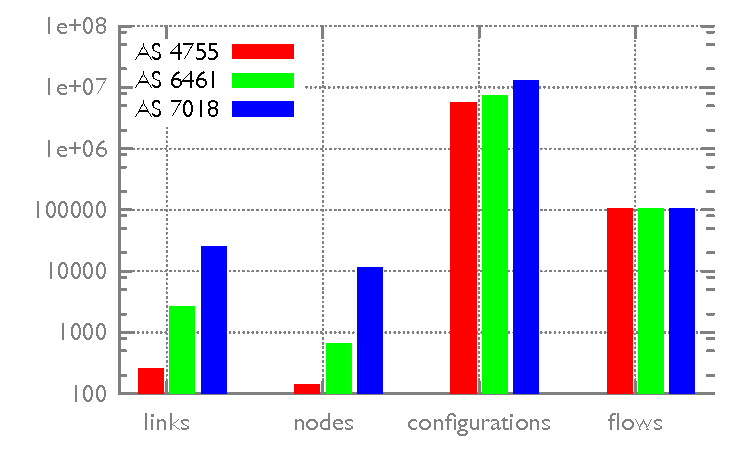
\includegraphics[width=1\linewidth]{figures/init.pdf}
  \caption{Configuration size.}
  \label{fig:init}
\end{figure}

\begin{figure}
  \centering
  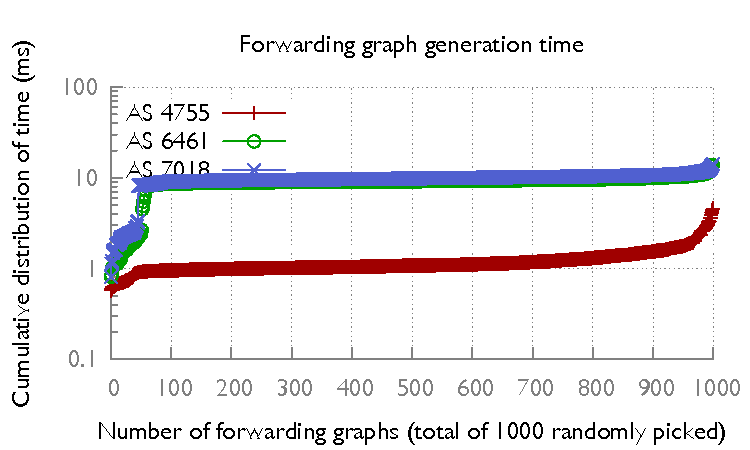
\includegraphics[width=1\linewidth]{figures/fg_cdf1000.pdf}
  \caption{Forwarding graph generation.}
  \label{fig:init}
\end{figure}

\begin{figure}
  \centering
  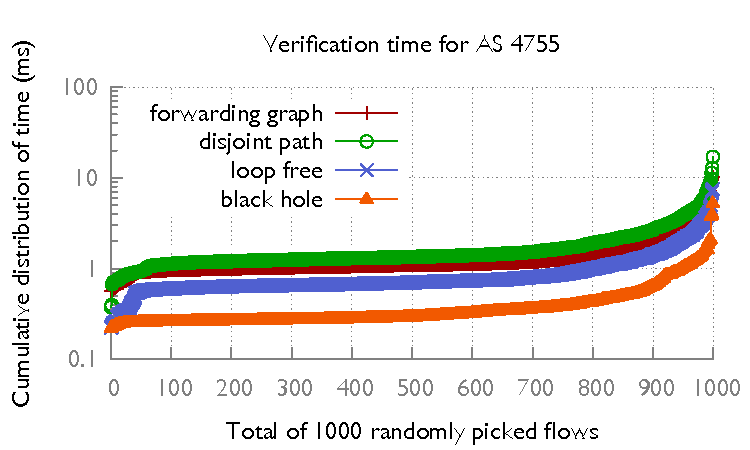
\includegraphics[width=1\linewidth]{figures/verify_cdf1000.pdf}
  \caption{Verification Time.}
  \label{fig:init}
\end{figure}

\begin{figure}
  \centering
  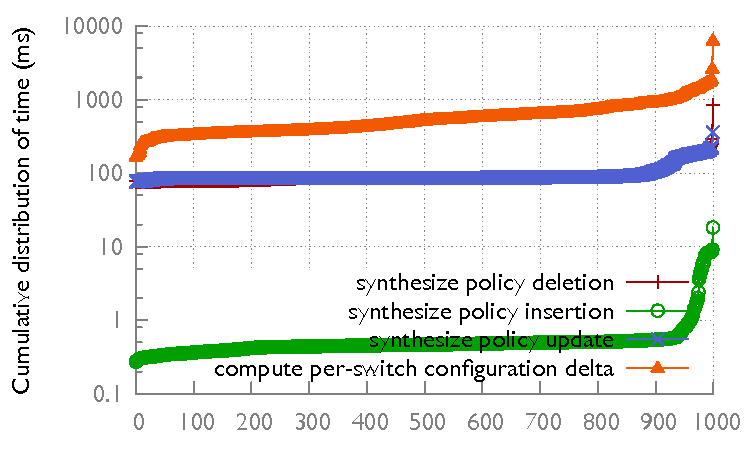
\includegraphics[width=1\linewidth]{figures/vn_synthesis_cdf1000.pdf}
  \caption{virtual network synthesis.}
  \label{fig:init}
\end{figure}

\begin{figure}
  \centering
  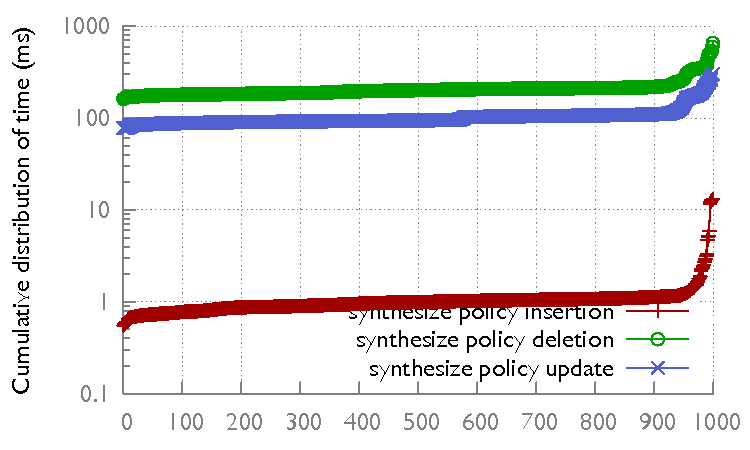
\includegraphics[width=1\linewidth]{figures/obs_synthesis_cdf1000.pdf}
  \caption{one-big-switch network synthesis (distributed firewall).}
  \label{fig:init}
\end{figure}

\subsection{Tradeoff: expressivenss, automation, and performance}

% \begin{figure*}
%   \centering
%   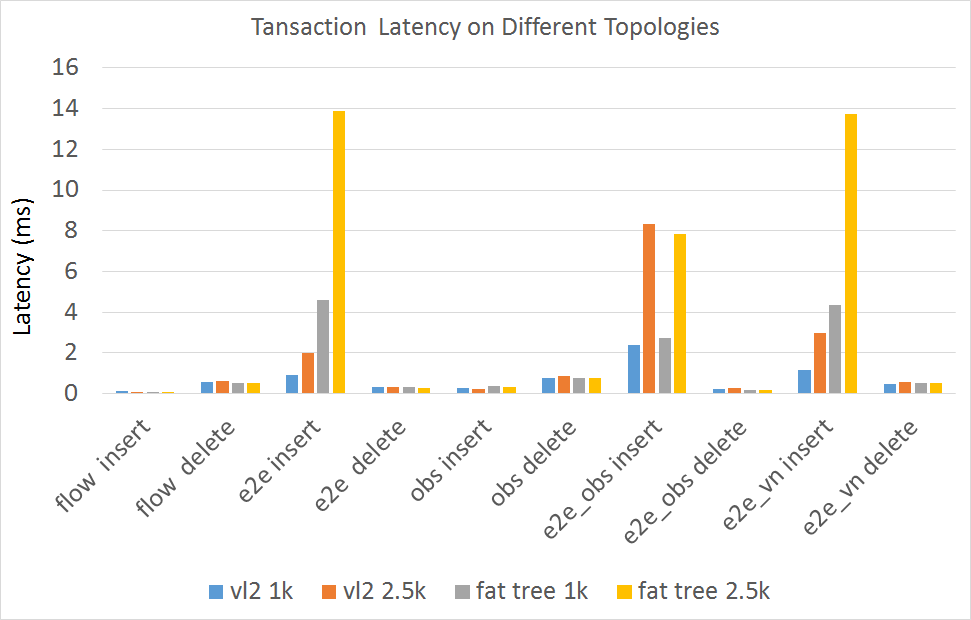
\includegraphics[width=1\linewidth]{transaction_latency.png}
%   \caption{Latency of transactions against different topologies.}
%   \label{fig:latency-all}
% \end{figure*}

% % GNUPLOT: LaTeX picture
\setlength{\unitlength}{0.240900pt}
\ifx\plotpoint\undefined\newsavebox{\plotpoint}\fi
\sbox{\plotpoint}{\rule[-0.200pt]{0.400pt}{0.400pt}}%
\begin{picture}(1500,900)(0,0)
\sbox{\plotpoint}{\rule[-0.200pt]{0.400pt}{0.400pt}}%
\put(151.0,146.0){\rule[-0.200pt]{4.818pt}{0.400pt}}
\put(131,146){\makebox(0,0)[r]{ 6}}
\put(1419.0,146.0){\rule[-0.200pt]{4.818pt}{0.400pt}}
\put(151.0,221.0){\rule[-0.200pt]{4.818pt}{0.400pt}}
\put(131,221){\makebox(0,0)[r]{ 7}}
\put(1419.0,221.0){\rule[-0.200pt]{4.818pt}{0.400pt}}
\put(151.0,296.0){\rule[-0.200pt]{4.818pt}{0.400pt}}
\put(131,296){\makebox(0,0)[r]{ 8}}
\put(1419.0,296.0){\rule[-0.200pt]{4.818pt}{0.400pt}}
\put(151.0,372.0){\rule[-0.200pt]{4.818pt}{0.400pt}}
\put(131,372){\makebox(0,0)[r]{ 9}}
\put(1419.0,372.0){\rule[-0.200pt]{4.818pt}{0.400pt}}
\put(151.0,447.0){\rule[-0.200pt]{4.818pt}{0.400pt}}
\put(131,447){\makebox(0,0)[r]{ 10}}
\put(1419.0,447.0){\rule[-0.200pt]{4.818pt}{0.400pt}}
\put(151.0,522.0){\rule[-0.200pt]{4.818pt}{0.400pt}}
\put(131,522){\makebox(0,0)[r]{ 11}}
\put(1419.0,522.0){\rule[-0.200pt]{4.818pt}{0.400pt}}
\put(151.0,598.0){\rule[-0.200pt]{4.818pt}{0.400pt}}
\put(131,598){\makebox(0,0)[r]{ 12}}
\put(1419.0,598.0){\rule[-0.200pt]{4.818pt}{0.400pt}}
\put(151.0,673.0){\rule[-0.200pt]{4.818pt}{0.400pt}}
\put(131,673){\makebox(0,0)[r]{ 13}}
\put(1419.0,673.0){\rule[-0.200pt]{4.818pt}{0.400pt}}
\put(151.0,748.0){\rule[-0.200pt]{4.818pt}{0.400pt}}
\put(131,748){\makebox(0,0)[r]{ 14}}
\put(1419.0,748.0){\rule[-0.200pt]{4.818pt}{0.400pt}}
\put(321.0,131.0){\rule[-0.200pt]{0.400pt}{4.818pt}}
\put(321,90){\makebox(0,0){ 1.2}}
\put(321.0,756.0){\rule[-0.200pt]{0.400pt}{4.818pt}}
\put(549.0,131.0){\rule[-0.200pt]{0.400pt}{4.818pt}}
\put(549,90){\makebox(0,0){ 1.4}}
\put(549.0,756.0){\rule[-0.200pt]{0.400pt}{4.818pt}}
\put(777.0,131.0){\rule[-0.200pt]{0.400pt}{4.818pt}}
\put(777,90){\makebox(0,0){ 1.6}}
\put(777.0,756.0){\rule[-0.200pt]{0.400pt}{4.818pt}}
\put(1004.0,131.0){\rule[-0.200pt]{0.400pt}{4.818pt}}
\put(1004,90){\makebox(0,0){ 1.8}}
\put(1004.0,756.0){\rule[-0.200pt]{0.400pt}{4.818pt}}
\put(1232.0,131.0){\rule[-0.200pt]{0.400pt}{4.818pt}}
\put(1232,90){\makebox(0,0){ 2}}
\put(1232.0,756.0){\rule[-0.200pt]{0.400pt}{4.818pt}}
\put(151.0,131.0){\rule[-0.200pt]{0.400pt}{155.380pt}}
\put(151.0,131.0){\rule[-0.200pt]{310.279pt}{0.400pt}}
\put(1439.0,131.0){\rule[-0.200pt]{0.400pt}{155.380pt}}
\put(151.0,776.0){\rule[-0.200pt]{310.279pt}{0.400pt}}
\put(30,453){\makebox(0,0){Counts}}
\put(795,29){\makebox(0,0){Times (ms)}}
\put(795,838){\makebox(0,0){Gnuplot Example}}
% \put(1279,736){\makebox(0,0)[r]{'exp.dat' u 1:2:(sqrt($2))}}
\put(1299.0,736.0){\rule[-0.200pt]{24.090pt}{0.400pt}}
\put(1299.0,726.0){\rule[-0.200pt]{0.400pt}{4.818pt}}
\put(1349,736){\makebox(0,0){$+$}}
\put(1399.0,726.0){\rule[-0.200pt]{0.400pt}{4.818pt}}
\put(151.0,131.0){\rule[-0.200pt]{0.400pt}{155.380pt}}
\put(151.0,131.0){\rule[-0.200pt]{310.279pt}{0.400pt}}
\put(1439.0,131.0){\rule[-0.200pt]{0.400pt}{155.380pt}}
\put(151.0,776.0){\rule[-0.200pt]{310.279pt}{0.400pt}}
\end{picture}


% \begin{figure*}[ht!]
%         \centering
%         \begin{subfigure}[b]{.4\linewidth}
%           \centering
%           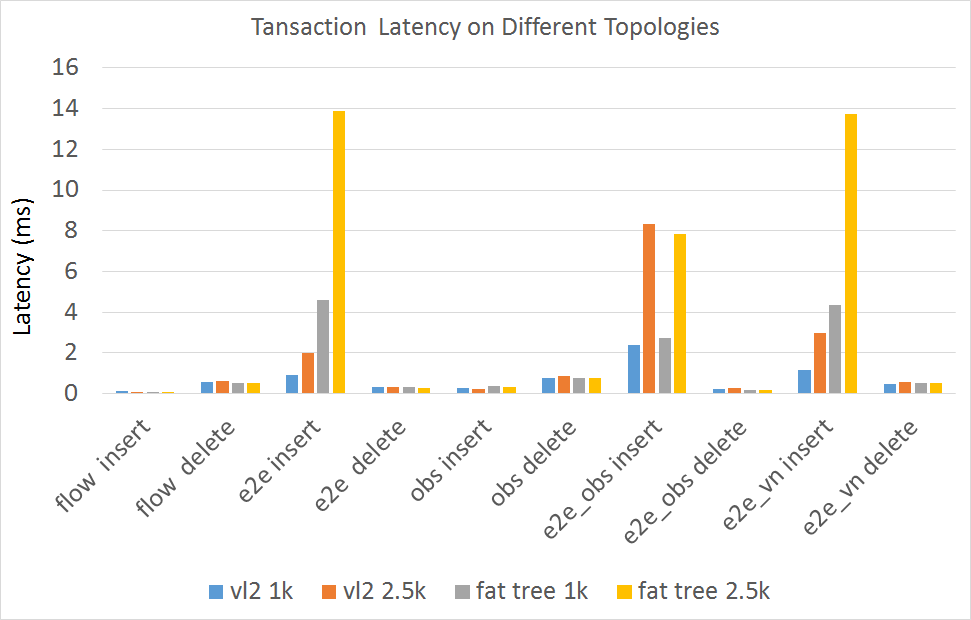
\includegraphics[width=1\textwidth]{transaction_latency.png}
%   \caption{Latency of transactions against different topologies.}
%   \label{fig:latency-all}
%           % \includegraphics[width=1\textwidth]{fig-SDNandDB-cropped.pdf}
%           % \caption{\textit{\textbf{SDN architecture (left)}},
%           %   \textit{\textbf{database architecture
%           %       (right)}}. \textit{\textbf{SDN networks}} offers a
%           %   centralized logical view of the network infrastructure:
%           %   app/users see the same complex network states, controller
%           %   carefully handles name/device binding;
%           %   \textit{\textbf{database}} bridges user and data by two
%           %   separate data abstractions: logical base tables hide
%           %   physical heterogeneity, external views interface end
%           %   users, \textbf{view maintenance and update} synchronize
%           %   the two.}
%           % \label{fig:SDNandDB}
%         \end{subfigure}
%         \hfill
%         \begin{subfigure}[b]{.232\linewidth}
%   \centering
%   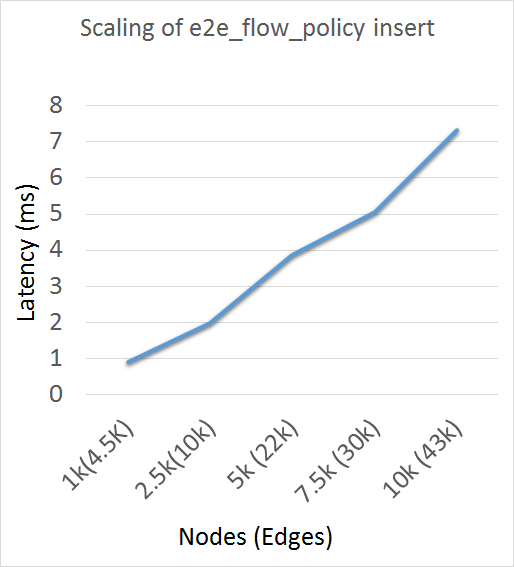
\includegraphics[width=1\textwidth]{scaling.png}
%   \caption{Latency against network size.}
%   \label{fig:trend}
%         \end{subfigure}
%         \begin{subfigure}[b]{.35\linewidth}
% \begin{center}
%     \small 
% \begin{tabular}{ | l | c | c |}
% \hline
% \textbf{operation} & \textbf{st (10ms)} & \textbf{ st (1s) }  \\
% \hline
% \hline
% flow insert  	 & 	91	&	9,091 \\
% \hline
% flow delete 	&	17	&	1,695 \\
% \hline
% e2e insert	& 16	&	1,563 \\
% \hline
% e2e delete   &  32	&	3,226 \\
% \hline
% obs insert	      & 	29	&	2,857 \\
% \hline
% obs  delete	&  16	&	1,587 \\
% \hline
% e2e\_obs insert	&  	15	&	1,471 \\
% \hline
% e2e\_obs delete & 	37	&	3,704 \\
% \hline
% e2e\_vn insert	&	23	&	2,273 \\
% \hline
% e2e\_vn delete	&	21	&	2,128 \\
% \hline
% \end{tabular}
% \end{center}
% 	\caption{STF measure for 100-node VL2 with 404 edges.\label{fig:stf}}
%   % \centering
%   % 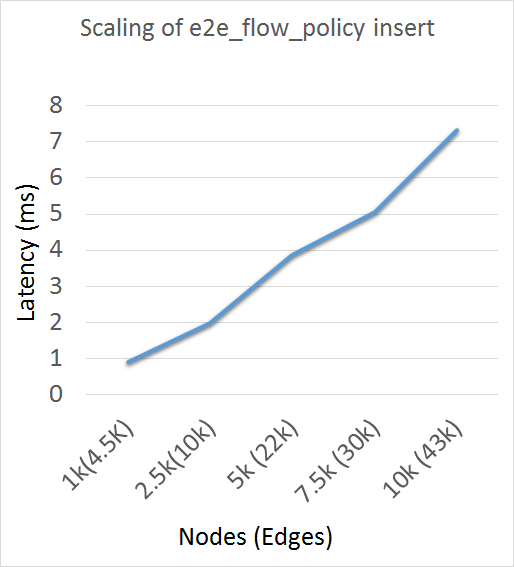
\includegraphics[width=1\textwidth]{scaling.png}
%   % \caption{Scaling of latency with network size.}
%   % \label{fig:trend}
%         \end{subfigure}
%         \caption{\footnotesize \Sys induced latency very small compared to the
%           switching rule update time}\label{fig:eval}
% \end{figure*}
% % \vspace{-3em}

% A prototype of several core features \TI demonstrates promising
% performance, showing that \Sys induced per-rule latency is less than
% 14 ms for all network instances up to 10k nodes, achieving very high
% STF (switch-time fraction) and linear growth as network size
% increases. 

% Specifically, Figure~\ref{fig:latency-all} summarizes the latency (in
% millisecond) induced by DB operation for each FIB update.  For each
% table in the x-axis: base table \nd{flow} (per-switch rule), view
% \nd{e2e} (end to end policy on physical network), \nd{obs}
% (one-big-switch configuration), \nd{obs\_e2e} (e2e policy for
% one-big-switch), and \nd{e2e\_vn} (e2e policy for virtual network), we
% run two operation, insert of a new record, and deletion of an existing
% one, where delay is computed on four networks, \nd{vl2 1k, 2.5k} (VL2
% topology with 1k and 2.5k nodes), and \nd{fat\_tree 1k, 2.5k}. The
% delay for all instances is on the scale of 1-14 ms. We also observe
% that inserts incur most noticeable delay for
% \nd{e2e,e2e\_obs,e2e\_vn}, since the \nd{e2e} view insert involves an
% extra step of path selection between the end nodes. In addition,
% Figure~\ref{fig:trend} shows the linear growth of \Sys induced latency
% as network size increases from 1k to 10k on VL2 topology.  And
% Figure~\ref{fig:stf} computes for each DB operation the switch time
% fraction (STF = $\frac{Switch\;\; time}{DB\; induced\; delay\; time}$)
% on 100-node VL2 network with switch time of 10ms (the average rule
% update time on a controlled network of 100 nodes~\cite{ffc}) and 1 sec
% (a representative time in B4 network~\cite{b4}).

% \begin{figure}[h]
% \begin{center}
%     \footnotesize
% \begin{tabular}{ | l | c | c |}
% \hline
% operation & st(10ms) & st(1s)  \\
% \hline
% \hline
% flow insert  	 & 	91	&	9,091 \\
% \hline
% flow delete 	&	17	&	1,695 \\
% \hline
% e2e insert	& 16	&	1,563 \\
% \hline
% e2e delete   &  32	&	3,226 \\
% \hline
% obs insert	      & 	29	&	2,857 \\
% \hline
% obs  delete	&  16	&	1,587 \\
% \hline
% e2e\_obs insert	&  	15	&	1,471 \\
% \hline
% e2e\_obs delete & 	37	&	3,704 \\
% \hline
% e2e\_vn insert	&	23	&	2,273 \\
% \hline
% e2e\_vn delete	&	21	&	2,128 \\
% \hline
% \end{tabular}
% \end{center}
% 	\caption{STF measure for 100-node vl2 with 404 edges.\label{fig:stf}}
% \end{figure}

